\section{Intel 486}

\begin{wrapfigure}[5]{r}{0.25\textwidth}
\centering
\includegraphics[width=.25\textwidth]{drawings/intel_logo.pdf}
\end{wrapfigure}

1989 年发布的 80486 是一次性能演进,解决了 80386 的所有瓶颈。然而它 950 美元(2018 年约 1,920 美元)的标价让大多数消费者望而却步。到 1993 年它终于变得可负担(约 500 美元),并成为 \doom{} 的推荐 CPU。\\
\par
与前代相比,设计发生了显著变化。流水线增加了两个额外阶段,深度扩展到五级。原本可选并位于主板某处的 FPU\footnote{Floating Point Unit.} 被集成到芯片内部。更重要的是,制造工艺的改进\footnote{1.0$\mu$ 工艺(相对 i386 的 1.5$\mu$)与更大的晶圆面积让晶体管数量提升到 120 万(i386 只有 275,000)。它是第一颗包含超过 100 万晶体管的 x86 芯片。}让 486 具备更复杂的设计,并首次集成了 L1 缓存——这是 Intel 在 386 上尝试但未成功的功能。\\
\par
\fq{386 其实有一块小缓存,后来被取消了,因为在芯片可容纳的缓存规模下性能不够。问题在于,如果把芯片做得更大,它会字面意义上放不进光刻机的视野里进行曝光。}{Gene Hill - Intel 386 Microprocessor Design and Development}\\
\par
{
\setlength{\belowcaptionskip}{-10pt}
\drawing{486_arch}{Intel 486 架构。}
}
\pagebreak
和 386 一样,Intel 将新 CPU 以两种型号进行市场推广。DX 版本是完整技术形态,而 SX 版本则禁用了 FPU。一个流传已久的顽固说法认为 DX/SX 的区分是 Intel 为了销售制造瑕疵芯片的营销伎俩。事实上这是有意的商业策略\footnote{来源:Michal Necasek 的《Lies, Damn Lies, and Wikipedia》;时间线不成立,因为“486DX 在 1989 年末已大规模出货,而 486SX 到 1991 年中才推出。在前 18 个月良率问题最严重的时期,根本没有 SX。”},用来提供 50\% 的折扣并出售 i487 FPU 协处理器。\footnote{有趣的是,i487 FPU 升级实际上是一颗完整的 486DX,会完全禁用 486SX!}。\\
\par
回头看,486 是 Intel 的 1994 年冠军,也是无可争议的强者(无论性能还是销量\footnote{截至 2015 年末,486 仍在生产并用于网络路由器。}),但它也经历了一段不确定时期。正如 386 需要面对兄弟(i960),i486 也要面对同公司挑战者——“Intel 860”。\\
\par
\fq{

\begin{wrapfigure}[11]{r}{0.55\textwidth}
\centering
\scaledimage{0.55}{i860.png}
\end{wrapfigure}

……我们当时几乎同时推出两款非常强大的芯片:以 CISC 技术为主、兼容所有 PC 软件的 486,以及基于 RISC 技术、速度很快但不兼容任何东西的 i860。我们不知道该怎么办,于是把两者都推出,打算让市场决定。然而事情没那么简单。支持一种微处理器架构及其配套产品——软件、销售与技术支持——需要巨量资源。即便是 Intel,也只能勉强把一套架构做到位。现在我们有两套不同且相互竞争的努力,每一套都不断吞噬更多内部资源。开发项目往往像寓言里的芥菜籽一样膨胀。资源之争与营销注意力之争(例如见客户时该强调哪款处理器)导致内部争论激烈到足以撕裂我们的微处理器组织。同时,我们的摇摆让客户怀疑 Intel 到底代表什么:486 还是 i860?}{Andy Grove, "Only the paranoid survive"}





在纸面上,i860 相当强大,是严肃对手。它采用重度流水线化的超标量架构,压榨 VLIW\footnote{Very Long Instruction Word.},拥有 X、Y、Z 三个单元并行处理,若使用得当可超越 Intel 486。\\
\par
但后来如 Pentium 等 CPU 选择隐藏芯片复杂性,通过硬件自动并行执行指令;而 i860 的架构要求直接操纵并行流水线。芯片不做幕后工作,完全依赖编译器作者按序安排指令。\\
\par
不幸的是,当时编译器技术尚未到位。没有 Intel 的全力支持来打造必要工具,现有编译器根本无法生成能利用其超标量能力的指令。i860 从未发挥出全部潜力。如果 Intel 当时愿意构建其迫切需要的工具,i860 的历史可能会不同。\\
\par
\par
\cscaledimage{0.85}{i486DX.png}{Intel 80486 封装。}
\par
图 \ref{i486DX.png} 展示了 Intel 486 的晶粒,内含 1,180,235 个晶体管。大约在这个时期,Intel 开始在 CPU 上印商标,以与日益强势的 AMD 与 Cyrix 克隆区隔。\\
\par
\trivia{i860 仍与 \doom{} 有关,因为它被用于 NeXTDimension 的视频处理板。}

\par
\subsection{流水线改进}
将 486 的 MIPS 性能与上一代对比,可以直观看到提升。得益于更好的制造工艺,顶级 486 可运行在 50MHz\footnote{为达到该频率,486 DX 50MHz 采用 1.0$\mu$ 工艺制造。},但频率提升并非主要原因。\\
\par
仔细观察图表会发现,即使在相同频率下,486 的处理能力也超过 386 的两倍。\\

\par
\begin{figure}[H]
\centering
  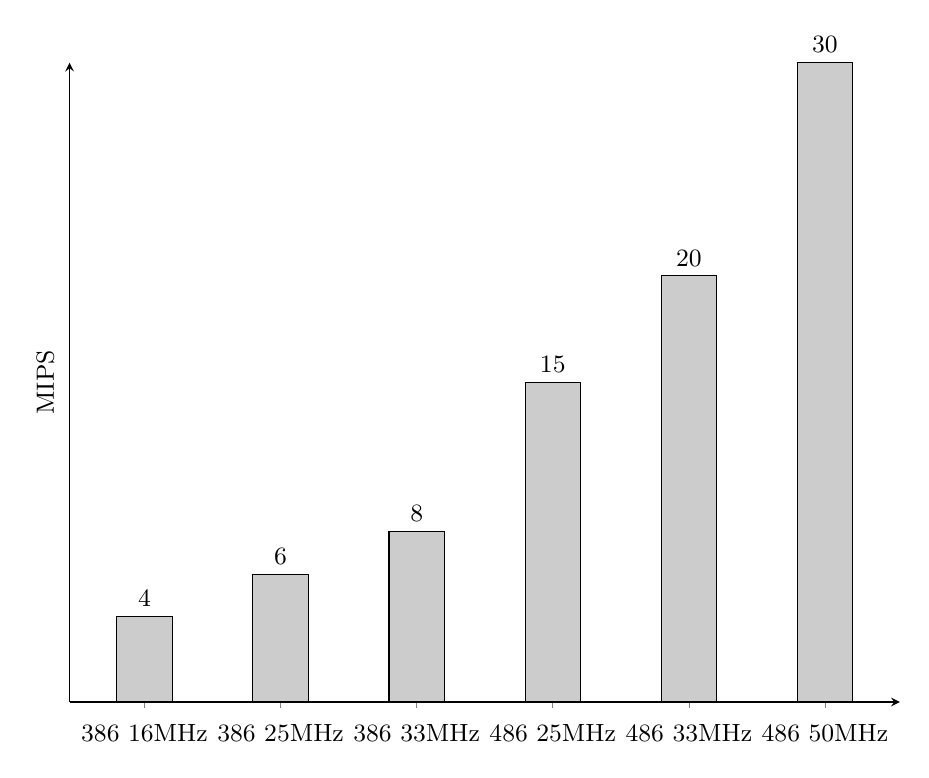
\begin{tikzpicture}[font=\small]
    \begin{axis}[
      width=1.0\textwidth,
      height=0.8\textwidth,
      ybar,
      bar width=20pt,
      ylabel={MIPS},
      ymin=0,
      ytick=\empty,
      xtick=data,
      axis x line=bottom,
      axis y line=left,
      enlarge x limits=0.11,
      symbolic x coords={386 16MHz,386 25MHz,386 33MHz,486 25MHz,486 33MHz,486 50MHz},
      xticklabel style={anchor=base,yshift=-\baselineskip},
      nodes near coords={\pgfmathprintnumber\pgfplotspointmeta}
    ]
      \addplot[fill=black!20,draw=black] coordinates {
        (386 16MHz,4)
        (386 25MHz,6)
        (386 33MHz,8)
        (486 25MHz,15)
        (486 33MHz,20)
        (486 50MHz,30)
      };
    \end{axis}
   
   \end{tikzpicture}
   \caption{Intel CPU 的 MIPS 对比\protect\footnotemark。}
 \end{figure}
\footnotetext{"每秒百万指令(MIPS)。来源:Roy Longbottom 的 PC Benchmark:http://www.roylongbottom.org.uk/mips.htm。"}

486 提升性能的方式是更高的平均吞吐量。其文档将 386 描述为三级流水线处理器。图 \ref{386_doc_pipeline} 显示在理想条件下,它应能每个周期执行一条指令。实际情况如图 \ref{386_real_pipeline},速度是理论的一半。

\begin{figure}[H]
\centering
\includegraphics[width=\textwidth]{drawings/386_instruction_pipeline.pdf}
\caption{根据 Intel 文档的 386 理论流水线。}
\label{386_doc_pipeline}
\end{figure}



\par
即使 Prefetch Unit 与 Execution Unit 供给充足,Decode 单元解码一条指令至少需要两个周期\footnote{由于 x86 使用变长指令,解码较复杂;而 RISC 采用定长指令。}。流水线最大吞吐量不能超过最慢阶段,因此 Intel 386 最多每两周期处理一条指令。\\
\par

\begin{figure}[H]
\centering
\includegraphics[width=\textwidth]{drawings/actual_386_instruction_pipeline.pdf}
\caption{实际 386 流水线:每条指令两个周期。}
\label{386_real_pipeline}
\end{figure}

\par
为解决该问题,Intel 将三级流水线拆成五级(Prefetch、Decode1、Decode2、Execute、WriteBack)。当所有阶段以 1 CPI\footnote{Cycle Per Instruction.} 运行时,486 的总吞吐量翻倍(只要流水线不被饿死)。\\
\par
\begin{figure}[H]
\centering
\includegraphics[width=\textwidth]{drawings/actual_486_instruction_pipeline.pdf}
\caption{486 流水线:每条指令一个周期。}
\end{figure}
\par





\subsection{缓存}
修改流水线并让每个阶段同速运行是正确方向的一步,但加深流水线也让它更容易饥饿。从空流水线开始,486 的延迟是 5 个周期,而 386 为 4 个周期。频繁停顿的 486 可能比 386 更慢。因缺少数据或指令而暂停处理必须尽量避免。\\
\par
从技术角度看,这是个几乎无解的问题。自 1980 年以来,RAM 性能落后于 CPU 性能。每年 CPU 性能提升 60\%,而 DRAM 只提升 7\%,差距每年扩大 50\%。到 1989 年,DRAM 访问时间比 CPU 周期慢 10 倍。\\
\par
\vspace{2mm}
\drawing{ram_vs_cpu}{来源:《Computer Organization and Design》Hennessy 与 Patterson}
\par
在 486 之前,CPU 请求 DRAM 中的指令或数据时,总要停下来,通过 Bus Unit 与主板内存控制器通信。即便 ISA 总线协议已很优化,至少也要两个周期。\\
\par 
第一个周期发起总线请求,置地址线并设置控制线(读/写)。随后进入等待周期(Intel 称之为 Wait State,因为 CPU 在等待 Bus Unit 时什么都不做),等待总线另一端的设备完成请求。\\
\par
\drawing{cpu_chipset_bus}{386 CPU-RAM 通信要素。}
\par
若设备能在第一个等待周期内响应,CPU 可达到零等待状态并继续运行。否则会插入额外 Wait State 直到完成。就性能而言,这些 Wait State 是灾难:不仅指令完成更慢,还会让流水线中其他指令全部停滞。\\
\par
\rawdrawing{cpu_wait_states}
\par
两周期总线请求已是 CPU 能达到的最快速度,而现实中 DRAM 访问需要多个 Wait State。
要避免这种情况,就要尽量避免使用总线。因此 Intel 在流水线与 Bus Unit 之间加入了 L1(一级)缓存。思路是利用程序的空间与时间局部性。\\
\par
时间局部性依赖程序的迭代特性:在循环中,最近访问的指令很可能在下一次迭代中再次访问。空间局部性与程序顺序读写数组的方式有关:访问某个地址后,附近地址很可能也会在不久后被访问。\\
\par
利用这两种特性,位于 CPU 与 Bus Unit 之间的良好缓存常常已包含所需数据或指令,使总线请求不再必要。\\
\par
\drawing{cpu_cache}{486 CPU-RAM 通信要素。}



\vspace{-20pt}
\subsection{L1 缓存}
现在希望已非常清楚:缓存是整个 CPU 的基石。设计缓存以获得尽可能高的命中率,并让它尽可能快,是至关重要的。

\subsubsection{DRAM vs SRAM}
缓存首先得益于更低的 RAM 延迟。主板 SIMM 槽中的主存使用 DRAM(动态 RAM),而缓存使用另一种更快的 SRAM(静态 RAM)。DRAM 典型访问时间约 200ns,而 SRAM 可达 20ns,快 10 倍。\\
\par
速度差来自于单元结构设计。\\
\par
DRAM 单元保存 1 bit,结构简单,包含一个晶体管和一个存储电容,便于高密度与大容量。然而电容会随时间漏电并在每次访问时损耗电荷。每次读取后必须写回;即便不访问也要每 15$\mu s$ 刷新一次。\\
\par
\scaleddrawing{1}{DRAM}{动态 RAM 及其保存 1 bit 的两种元素。}
\vspace{-5pt}
慢的原因是每个单元维护成本高。DRAM 还远离 CPU,位于主板某处,需要使用与其他设备共享的 ISA 总线。\\
\par

\vspace{2mm}
更复杂的设计(密度较低、制造更贵)让 SRAM 单元没有这些缺点。\\
\par
\scaleddrawing{1}{SRAM}{由六个元素构成的静态 RAM。}
\par
没有电容,SRAM 单元不会漏电,不需要周期刷新,也无需每次访问后写回。它的两条位线使电压变化检测速度翻倍,时序更快。因为位于 CPU 芯片内部,访问不需昂贵总线请求,也不存在与其他设备的争用\footnote{DRAM 速度后来提升。Fast Page Mode 通过 SDRAM 行缓冲缓存 DRAM 行。udacity.com 的 UPCF 课程非常适合深入了解该主题。}。
\par







\subsubsection{缓存行}
L1 缓存不仅硬件更好,设计也很巧妙。其容量很小(8 KiB)且负载很重(代码与数据统一缓存),压力不小,却在正常运行时实现了 92\% 的命中率\footnote{来源:《The i486 CPU: Executing Instructions in One Clock Cycle》。}。\\
\par
为实现这一点,Intel 工程师采用四路组相联设计,将 $2^{32}$ 地址空间划分为 2,097,152 个 2 KiB 页。每页包含 128 条 16 字节的缓存行(cachelines)。\\
\par
\drawing{cacheline}{一个缓存行的 16 字节。}
\par
缓存系统由一个目录和四个 bank(也称 ways)组成。每个 way 可存储 128 条 16 字节缓存行,总容量 2 KiB。这些 16 字节行是缓存的基本单位。\\
\drawing{mem_to_way}{缓存控制器如何解释内存地址。}
\par
收到 32 位地址访问请求后,缓存控制器将其拆分为图 \ref{mem_to_way} 所示的三个字段,并执行如下步骤。
\begin{enumerate}
\item 使用 LINE 字段 [4-10] 查找 128 个目录项之一。
\item 查看该目录项中的四个 tag。若有一个与 TAG [11-31] 匹配,则说明缓存行存在于四个 way 之一。
\item 检查目录项中的标志位 F,确保缓存行有效。
\item 使用 OFFSET [0-3] 字段访问缓存行中的 16 个值之一。
\item 更新目录项的 F 标志以更新 LRU\footnote{Least Recently Used.} 值。
\end{enumerate}
\par
一个内存地址的内容可以在四个 way 的任意一个中,但 LINE 偏移总是相同。由于 $2^{32} / 128 = 33,554,432$ 个地址竞争四个槽位,不可避免的缓存行淘汰由 LRU 策略裁决\footnote{淘汰可发生在读或写时,若缓存为 write-allocate(所有 Intel 486 都是如此)。来源:《Internal Cache Architecture of X86 Processors》。}。\\
\par
\drawing{cacheways}{缓存控制器与四个 way(bank)。}
\par
\trivia{如果增加 way 数或缓存大小会怎样?在 8 KiB 缓存下,四路是最优折中\footnote{来源:《Computer Architecture: A Quantitative Approach》Hennessy/Patterson。}。两路缓存的 miss 率为 14\%,四路为 10.5\%。提高到八路只改善到 10\%,全相联也只有 9\%。}\\
\par

\rawscaleddrawing{0.9}{set_state_caches}



\subsection{总线突发传输}
486 流水线中的任何缓存未命中都会触发缓存行淘汰,并需要将完整 16 字节从 DRAM 传输到 SRAM\footnote{预取器也以 16 字节为单位工作,将缓存行取入 32 字节预取队列。}。这通常是成本高昂且对 CPU 非常不利的操作。但 Intel 增加了所谓 “Burst Transfer” 能力,使其协同运作。\\
\par
原理很简单:在等待数据到达时,锁存下一次请求,这样总线控制器可以立即使用它,而不必等待 CPU 初始化新的总线请求。\\
\par
\drawing{netburst}{“Burst Transfer” 让缓存行填充速度提高 65\%。}






\subsection{Overdrive 与 L1 写回}
Intel 通过 80486 OverDrive 系列让性能提升 33\%。这些 CPU 带有倍频器,使其运行频率是总线的两倍(33MHz 型号运行在 66MHz)\footnote{直到今天,设计者仍在解决 CPU 远快于总线的问题。}。此外,L1 缓存策略变为写回(而非写直达),显著降低了总线流量。\\
\par 
\vspace{10pt}
\scaleddrawing{0.9}{486dx2_notm}{“DX2-66” 是运行 \doom{} 的黄金标准与最佳选择}%{Best CPU to run \doom at the time.}
\par
%\trivia{Want even more performance? Not only a DX2-66 ran faster, they also came with an enhanced writeback L1 cache\footnote{The standard 486 L1 cache was writethrough with post-writes.}}

\begin{figure}[H]
\centering
  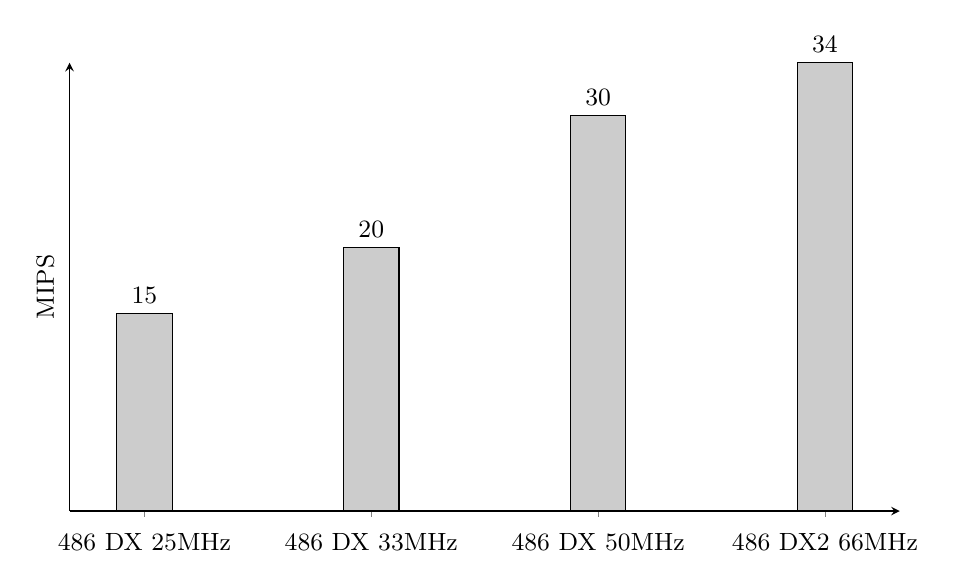
\begin{tikzpicture}[font=\small]
    \begin{axis}[
      width=1.0\textwidth,
      height=0.6\textwidth,
      ybar,
      bar width=20pt,
      ylabel={MIPS},
      ymin=0,
      ytick=\empty,
      xtick=data,
      axis x line=bottom,
      axis y line=left,
      enlarge x limits=0.11,
      symbolic x coords={486 DX 25MHz,486 DX 33MHz,486 DX 50MHz,486 DX2 66MHz},
      xticklabel style={anchor=base,yshift=-\baselineskip},
      nodes near coords={\pgfmathprintnumber\pgfplotspointmeta}
    ]
      \addplot[fill=black!20,draw=black] coordinates {
        (486 DX 25MHz,15)
        (486 DX 33MHz,20)
        (486 DX 50MHz,30)
        (486 DX2 66MHz,34)
      };
    \end{axis}
   
   \end{tikzpicture}
   \caption{CPU 的 MIPS 对比\protect\footnotemark。}
 \end{figure}
\footnotetext{来源:“Roy Longbottom's PC Benchmark Collection: http://www.roylongbottom.org.uk/mips.htm”。}
\par
注意图中 486DX2-66MHz 比 486DX-50MHz 更快,但并没有频率带来的 20\% 全部优势。这是因为 DX2 的总线运行在 33MHz,而 DX 版本 CPU 与总线都运行在 50MHz。




\subsection{晶粒}
%To close this section on the 486, I cannot resist including a magnified photography of the die. 
如果你手里拿的是 9.25''x7.5'' 的实体书,CPU 封装边长为 30mm,晶粒尺寸为 15.5 x 9.9 mm,均以 1:1 比例展示。\\
\par
\bigskip

  \begin{figure}[!htb]

\begin{minipage}{0.48\textwidth}
\centering
\scaledrawimage{44.45mm}{486topdown.png}
%\caption{468 packaging.}
\end{minipage}
\hfill
\begin{minipage}{0.48\textwidth}
\centering
\includegraphics[width=44.45mm]{drawings/486toscale.pdf}
%\caption{The die inside the package.}
\end{minipage}
\end{figure}

\par



\begin{figure}[H]
\centering
\scaledimage{0.9}{486_blueprint.png}
\end{figure}
\par
\begin{figure}[H]
\centering
\scaledimage{0.9}{486_layout.png}
\end{figure}





\trivia{上一页的晶体管布局在数据通路与控制通路之间有所不同:数据通路为手工布线,控制通路使用专为 486 构建的 CAD 工具生成\footnote{来源:Coping with the Complexity of Microprocessor Design at Intel -- A CAD History。}。}\\
\par
\subsection{为 486 编程}
了解架构后,我们就能明白程序员如何充分利用 486。好消息是,大部分性能提升都属于 90 年代“白捡的午餐”。同样的二进制在新 CPU 上可快一倍。\\
\par
除了少数特殊情况\footnote{"Pushing the 486" by Michael Abrash.},只要程序员关注缓存行、最大化时间与空间局部性\footnote{并避免分支。没有分支预测器时,\cw{jmp} 会被忽略并通常带来两个周期的停顿。},CPU 处理整数就会飞快。浮点运算相较 i386 的 FPU(i387)提升了 2 倍。事实上提升如此之大,以至于 i487 的 \cw{FMUL} 比 i386 的 \cw{IMUL} 还快。\\
\par
\begin{figure}[H]
\centering
\begin{tabularx}{\textwidth}{ X  X X  X  X}
  \toprule
  \textbf{CPU} & \textbf{FADD} & \textbf{FMUL} & \textbf{FDIV} &\textbf{FXCH} \\
  \toprule
Intel 387 & 23-34 & 29-57   & 88-91 & 18 \\
Intel 487 & 8-20  & 16   & 73 & 4 \\ \bottomrule
\end{tabularx}
\caption{FPU 每条指令的周期数:387 vs 487。}

\end{figure}

\par
但 FPU 性能仍远不及 ALU 与其桶形移位器,因此 \doom{} 必须完全使用整数运算\footnote{游戏中浮点运算的曙光始于 1996 年 Intel Pentium 与 Quake。}。\\

\par
 \begin{figure}[H]
\centering  
\begin{tabularx}{\textwidth}{ L{0.25} L{0.25} L{0.25} L{0.25} }
  \toprule
  \textbf{CPU} &  \textbf{ADD}  & \textbf{MUL} & \textbf{DIV}\\
  \toprule 
   i487 (FPU) & 8-20  & 16 & 73\\
   i486 (ALU) & 1  & 12-42 & 43\\
   \toprule
\end{tabularx}
\caption{每条指令的周期数:ALU vs FPU。}
\end{figure}

%  \begin{figure}[H]
% \centering  
% \begin{tabularx}{\textwidth}{ L{0.3} L{0.3} L{0.4}}
%   \toprule
%   \textbf{Operation} &  \textbf{i486 (ALU)} & \textbf{i487 (FPU)} \\
%   \toprule 
%   
%    \cw{ADD} & 1 & 8-20\\
%    \cw{DIV} & 43 & 73\\
%    \cw{MUL} & 12-42 & 29-52\\
%    \toprule
% \end{tabularx}
% \caption{Cycles per instruction of ALU vs FPU.}
% \end{figure}

\par
\trivia{获取信息困难导致了关于 \doom{} 与浮点单元的各种传言。1994 年 \cw{alt.games.doom} 上一条“486DX 运行 Doom 是否比 SX 更快?”的长帖有助于了解当时的状况。主题在 1994 年 7 月发布,下面是(筛选后的)五条回复,足以说明接近真相有多难。}


\fq{\cw{我的朋友在买电脑,觉得没什么必要买 DX。有什么意见?(或硬证据 :) ?)。}}{\cw{Dave Gates@bestsd.sdsu.edu - 23 Jul 1994 05:28}}


\vspace{1mm}

\fq{\cw{DOOM 在 486DX/33 上运行 *快得多*,比 486SX/33。相信我,我在同一个房间看过两台机器。} }{\cw{BillyBoB 4@aol.com - 23 Jul 1994 10:45}}

\vspace{1mm}

\fq{\cw{就 CPU 速度而言它们 *没有* 区别。原因 DX 更快可能是 SX 的 ISA 显卡、没有缓存或内存更少。Doom 并不使用 FPU(数学协处理器),所以 SX 不会减速。}}{\cw{Chad Anson@daisy.cc.utexas.edu - 23 Jul 1994 11:48}}

\vspace{1mm}

\fq{\cw{我们有一台 486SX/25 和一台 486DX/50,DX 50 全屏高细节运行比 SX 的邮票大小还快。SX 慢到几乎不可玩。} }{\cw{BonesBro@aol.com - 23 Jul 1994 12:36}}

\vspace{1mm}

\fq{\cw{对于大多数 CPU 密集型应用与游戏(包括 DOOM),SX 明显比 DX 慢。}}{\cw{Neal W.Miller@@rebecca.its.rpi.edu - 23 Jul 1994 13:34}}

\vspace{1mm}


\fq{\cw{这不对!
486 SX 运行 Doom 的速度和 486 DX 完全一样
(如果使用相同的 VGA 卡和主板)。}}{\cw{Grassl Wolfgang@papin.HRZ.Uni-Marburg.DE - 23 Jul 1994 14:24}}






